%!TEX root = ../main.tex

\graphicspath{{./figures/introduction/}}

\chapter{FISH-based transcriptomics}
\label{ch:introduction}

\minitoc
\newpage

\section{Gene expression process}
\label{sec:gene_expression}

Cells are the basic unit of all living organisms.
Yet, a diversity of cell-type exists, performing different actions.
Some of those are common among all cells (cell division for example), but others can be very specific.
Most of the time, different cell-types perform diverse actions through a different set of functional molecules.
In order to implement these different cellular processes and to fulfill the variety of diverse functions, a cell gets its instructions from the \ac{DNA}.
The latter contains all the cell's genetic information and it is common for all cells of the same organism.
A \ac{DNA} strand presents a succession of genes, defined as long sequences of nucleotides.
They are organics molecules composed of a five-carbon sugar, a phosphate group and one of the four nucleobases: Adenine, Cytosine, Guanine and Thymine.
Together, these nucleobases form a genetic alphabet of 4 letters (A, C, G and  T).
Each gene encodes the blueprint of a functional molecule with a specific sequence of nucleobases.

Gene expression is the process by which genetic information is transformed into functional products.
\ac{RNA} molecules, or transcripts, are essential for this process.
They are either the functional gene products themselves or they serve as an intermediate molecule prior to the production of other functional products, namely the proteins.
A change in gene expression gives cells enough flexibility to adapt and react to different external stimuli.
It also drives cells differentiation, allows them to run their basic functions, modulate their activities and therefore appears to be one of the most fundamental processes of life.
On the contrary, its deregulation can lead to various diseases.
This explains the interest of the scientific community to study and decode gene expression processes.

In the living world, cells can be divided in two categories: prokaryotic cells and eukaryotic cells.
The prokaryotic cells, which do not have a nucleus and typically form a unicellular organism, and the eukaryotic cells, with a well-organized nucleus.
An eukaryote (a living organism with eukaryotic cells) is usually composed of cells with a higher level of compartmentalization through membrane-bound organelles.
The nucleus is obviously the most important of these organelles, with the \ac{DNA} inside.
The rest of the organelles are located in the cytoplasm, such as the mitochondria, the lysosomes, or the Golgi apparatus (see Figure~\ref{fig:eukaryotic_cell}).

For an eukaryote cell, the expression of a gene includes two main steps: the transcription of a \ac{DNA} sequence into a \ac{RNA} (in the nucleus) and the translation of a \ac{RNA} into a protein.
Between these two major steps, there is a phase of maturation for the transcript, before a potential exports outside the nucleus and a transport somewhere in the cytoplasm.
A cell can regulate either the transcription or the translation step to control the production of its functional molecules and thereby the biological process to which the proteins or \ac{RNA} contribute\footnote{For a complete and general introduction about cellular biology, an interested reader could see~\cite{alberts_molecular_2017}.}.

\begin{figure}[]
    \centering
    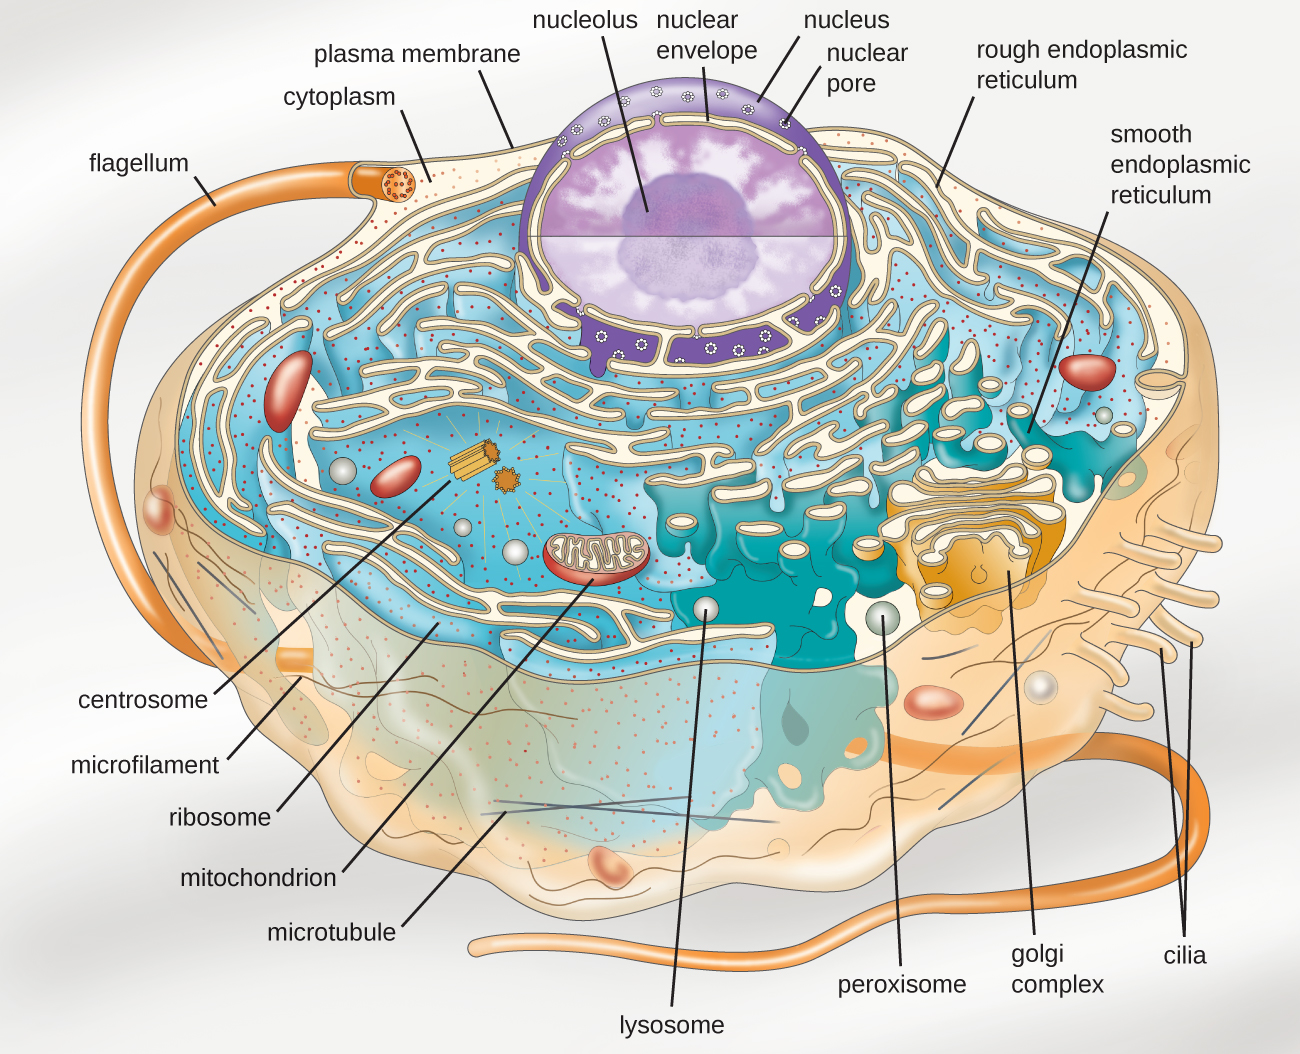
\includegraphics[width=0.8\textwidth]{figures/introduction/cell_eukaryotic.jpg}
    \caption[Eukariotic cell]{Illustration of an eukaryotic cell, from~\cite{parker2017microbiology}}
    \label{fig:eukaryotic_cell}
\end{figure}

\subsection{Transcription}
\label{subsec:intro_transcription}

\subsubsection{The primary transcripts}

This step consists in copying a gene (a sequence of nucleotides along the \ac{DNA} strands) into another biomolecules composed of nucleotides: a \ac{RNA}.
While the \ac{DNA} is stuck within the nucleus, the \ac{RNA} can convey the blueprint of the future protein outside.
In many cases, \ac{RNA} can be non-coding (they do not lead to the synthesis of a protein) and fulfill a variety of functions itself, for instance the regulation of gene expression.
In a \ac{RNA}, the nucleotide Uracil (U) replaces the Thymine (T) and a ribose sugar serves as backbone instead of a desoxyribose sugar.
If both \ac{DNA} and \ac{RNA} contain genetic information, \ac{RNA} is a shorter single-stranded molecule, compared to the double-stranded \ac{DNA}, and, therefore, is less stable.
However, they both have two distinctive ends 5' and 3' (corresponding to the number of carbon atoms in their sugar backbone extremities).\\

\noindent
Transcription proceeds as follows:
\begin{enumerate}
	\setlength\itemsep{0.1em}
	\item Proteins that serve as transcription factors bind to a specific sequence of \ac{DNA} (the promoter sequence) and recruit an enzyme (the \ac{RNA} polymerase) to initiate the transcription.
	\item The \ac{RNA} polymerase breaks the hydrogen bounds between the two \ac{DNA} strands to separate them.
	\item The \ac{RNA} polymerase moves along one \ac{DNA} strand, from 3' to 5' extremity, synthesizing a complementary nucleotides sequence on the way.
	\item The \ac{RNA} polymerase disengages from the strand when it meets a specific sequence of \ac{DNA} (the terminator sequence) and the newly synthesized nucleotides sequence (the primary transcribed \ac{RNA}) is released.
\end{enumerate}

\noindent
At this point, different sorts of \ac{RNA} are transcribed, depending of \ac{RNA} polymerase recruited:
\begin{itemize}
	\setlength\itemsep{0.1em}
	\item \ac{mRNA}, composed of coding (exon) and non-coding (intron) nucleotides, which conveys the blueprint of a future protein.
	\item \ac{rRNA} which, associated with ribosomal proteins, forms ribosomes, a macromolecular machine used by the cell to synthesize proteins.
	\item \ac{tRNA}, the most abundant \ac{RNA} molecule, which carries amino acids to the ribosome.
\end{itemize}

\subsubsection{RNA maturation}

For the rest of the manuscript, I mainly focus on the \ac{mRNA}s.
They do not fit translation requirements yet and need to undergo three processes before leaving the nucleus: the 5' end is transformed (\textbf{\ac{RNA} capping}), a poly(A) tail (repeated adenine-based molecules) is added at the 3' end (\textbf{polyadenylation}), then the non-coding parts of the \ac{RNA} sequence are removed (\textbf{splicing}).
Those transformations allow to move the \ac{mRNA} out of the nucleus, regulate its degradation and promote the translation.

\begin{figure}[]
    \centering
    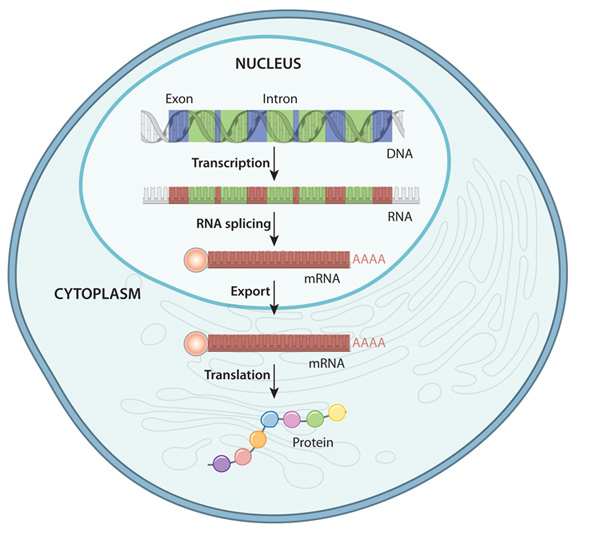
\includegraphics[width=0.8\textwidth]{figures/introduction/gene_expression_process.jpg}
    \caption[Gene expression process]{Overview of gene expression process, from~\cite{cell_essential_nature}}
    \label{fig:gene_expression}
\end{figure}

%%%%%%%%%%%%%%%%%%%%%%%%%%%%%%%%%%%%%%%%%%%%%%%%%%%%%%%%%%%%%%%%%%%%%%%%%%%%%%%%%%%%%%%%%%%%%%%%%%%%%%%%%%%%%%%%%%%%%%%%%%%%%%%%%%%%%%%%%%%%%%%%%%%%%%%%%%%%
%%%%%%%%%%%%%%%%%%%%%%%%%%%%%%%%%%%%%%%%%%%%%%%%%%%%%%%%%%%%%%%%%%%%%%%%%%%%%%%%%%%%%%%%%%%%%%%%%%%%%%%%%%%%%%%%%%%%%%%%%%%%%%%%%%%%%%%%%%%%%%%%%%%%%%%%%%%%
%%%%%%%%%%%%%%%%%%%%%%%%%%%%%%%%%%%%%%%%%%%%%%%%%%%%%%%%%%%%%%%%%%%%%%%%%%%%%%%%%%%%%%%%%%%%%%%%%%%%%%%%%%%%%%%%%%%%%%%%%%%%%%%%%%%%%%%%%%%%%%%%%%%%%%%%%%%%

\subsection{RNA transport mechanisms}
\label{subsec:intro_rna_transport}

When an \ac{mRNA} is ready for export, it is moved out of the nucleus through the nuclear pore complex.
This complex recognizes a mature \ac{mRNA} if a specific set of proteins is bounded to it (poly(a) binding proteins, cap binding proteins, and proteins related to the splicing step).
Once in the cytoplasm, an \ac{mRNA} is not necessarily exploited by a ribosome for translation.
It can also be silenced by translational repressors and stored, transported in a specific region of the cell or degraded.

Until recently, the scientific community thought translation mostly occurred at the endoplasmic reticulum and then proteins were transported where they were needed.
New evidence suggests on the contrary that \ac{mRNA} localization within the cell is not always random and \ac{mRNA}s-proteins colocalization could be an important aspect of cell organization and gene expression regulation \cite{Lecuyer2007}.
However, the involved mechanisms are not well understood yet and the extend of \ac{mRNA}s concerned by a specific localization pattern is still unknown.
Beyond the number of \ac{mRNA} molecules within a cell (the expression level of a gene), researchers manifest now an increasing interest for \ac{mRNA} localization.

\noindent
Some mechanisms used by the cell to transport or locally enrich \ac{mRNA} have already been identified:
\begin{itemize}
	\item Usage of motor proteins to move the \ac{mRNA}s along the cytoskeleton.
	\item Prevention of \ac{mRNA} degradation at a precise location.
	\item Local entrapment to anchor the \ac{mRNA}s.
\end{itemize}

%\begin{figure}[]
%    \centering
%    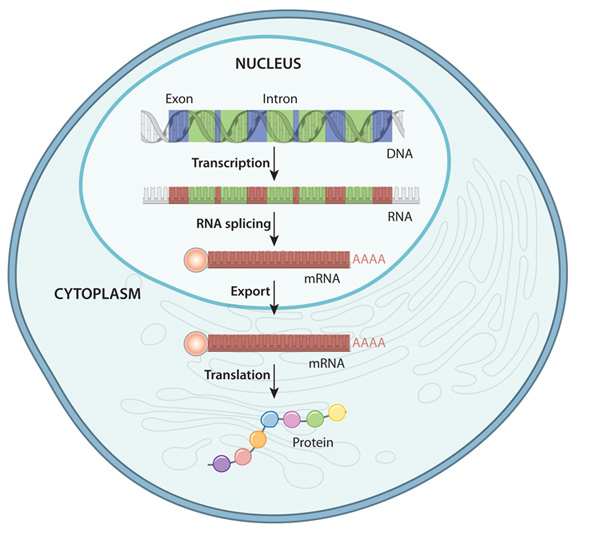
\includegraphics[width=0.8\textwidth]{figures/introduction/gene_expression_process.jpg}
%    \caption[Gene expression process]{Overview of gene expression process, from~\cite{cell_essential_nature}}
%    \label{fig:gene_expression}
%\end{figure}

%~\cite{das_intracellular_2021}

% google
% Ribonucleoprotein (RNP) granules are non-membrane bound compartments that form from RNA molecules and
% RNA-binding proteins. Different classes of RNPs carry out diverse roles: for example, some can regulate gene expression while another (the nucleolus) produces ribosomes.

%%%%%%%%%%%%%%%%%%%%%%%%%%%%%%%%%%%%%%%%%%%%%%%%%%%%%%%%%%%%%%%%%%%%%%%%%%%%%%%%%%%%%%%%%%%%%%%%%%%%%%%%%%%%%%%%%%%%%%%%%%%%%%%%%%%%%%%%%%%%%%%%%%%%%%%%%%%%
%%%%%%%%%%%%%%%%%%%%%%%%%%%%%%%%%%%%%%%%%%%%%%%%%%%%%%%%%%%%%%%%%%%%%%%%%%%%%%%%%%%%%%%%%%%%%%%%%%%%%%%%%%%%%%%%%%%%%%%%%%%%%%%%%%%%%%%%%%%%%%%%%%%%%%%%%%%%
%%%%%%%%%%%%%%%%%%%%%%%%%%%%%%%%%%%%%%%%%%%%%%%%%%%%%%%%%%%%%%%%%%%%%%%%%%%%%%%%%%%%%%%%%%%%%%%%%%%%%%%%%%%%%%%%%%%%%%%%%%%%%%%%%%%%%%%%%%%%%%%%%%%%%%%%%%%%

\subsection{Translation}
\label{subsec:intro_translation}

Finally, a cell synthesizes a protein through the translation process.
A ribosome is assembled around a \ac{mRNA} and moves along its nucleotides.
At the same time, \ac{tRNA}s carry amino acids matching the \ac{mRNA} sequence.
According to the genetic code, three successive nucleotides of the \ac{mRNA} (a codon) correspond to an amino acid.
The ribosome sequentially chains the amino acids, which then fold into a functional protein with a specific 3-dimensional structure.

%%%%%%%%%%%%%%%%%%%%%%%%%%%%%%%%%%%%%%%%%%%%%%%%%%%%%%%%%%%%%%%%%%%%%%%%%%%%%%%%%%%%%%%%%%%%%%%%%%%%%%%%%%%%%%%%%%%%%%%%%%%%%%%%%%%%%%%%%%%%%%%%%%%%%%%%%%%%
%%%%%%%%%%%%%%%%%%%%%%%%%%%%%%%%%%%%%%%%%%%%%%%%%%%%%%%%%%%%%%%%%%%%%%%%%%%%%%%%%%%%%%%%%%%%%%%%%%%%%%%%%%%%%%%%%%%%%%%%%%%%%%%%%%%%%%%%%%%%%%%%%%%%%%%%%%%%
%%%%%%%%%%%%%%%%%%%%%%%%%%%%%%%%%%%%%%%%%%%%%%%%%%%%%%%%%%%%%%%%%%%%%%%%%%%%%%%%%%%%%%%%%%%%%%%%%%%%%%%%%%%%%%%%%%%%%%%%%%%%%%%%%%%%%%%%%%%%%%%%%%%%%%%%%%%%

\subsection{mRNA localization}
\label{subsec:intro_rna_loc}

%%%%%%%%%%%%%%%%%%%%%%%%%%%%%%%%%%%%%%%%%%%%%%%%%%%%%%%%%%%%%%%%%%%%%%%%%%%%%%%%%%%%%%%%%%%%%%%%%%%%%%%%%%%%%%%%%%%%%%%%%%%%%%%%%%%%%%%%%%%%%%%%%%%%%%%%%%%%

%~\cite{Medioni_2012}

% Transporting mRNAs rather than proteins presents several significant advantages for a cell.
% First, transport costs are reduced, as several protein molecules can be translated from a single RNA molecule.
% Second, transporting mRNAs can prevent proteins from acting ectopically before they reach the appropriate site,
% which is particularly important in the case of maternal determinants, as spatially inappropriate expression disrupts embryonic patterning.
% Third, localized translation can facilitate incorporation of proteins into macromolecular complexes by generating high local
% protein concentrations and allowing co-translation of different subunits (Mingle et al., 2005).
% Fourth, nascent proteins may have properties distinct from pre-existing copies, by virtue of post-translational
% modifications or through chaperone-aided folding pathways (Lin and Holt, 2007).
% Lastly, a major advantage of mRNA targeting is that it allows fine-tuning of gene expression in both space and time.
% Examples of this include targeting of different splice variants to distinct cellular compartments (Baj et al., 2011)
% and activation of localized mRNA translation specifically at their destination, in response to signals
% such as guidance cues, neurotransmitter release or fertilization (Besse and Ephrussi, 2008).

%%%%%%%%%%%%%%%%%%%%%%%%%%%%%%%%%%%%%%%%%%%%%%%%%%%%%%%%%%%%%%%%%%%%%%%%%%%%%%%%%%%%%%%%%%%%%%%%%%%%%%%%%%%%%%%%%%%%%%%%%%%%%%%%%%%%%%%%%%%%%%%%%%%%%%%%%%%%

% chpater 5 intro racha

% Most of \ac{mRNA}s have a random distribution throughout the cytoplasm, but some localize in specific subcellular regions~\cite{Blower_2013, Jung_2014, Eliscovich_2017, Bovaird_2018}.

% Such localization can be related to either \ac{RNA} metabolism, for example with untranslated \ac{mRNA}s stored and repressed in \ac{P-bodies} (but not degraded~\cite{Hubstenberger_2017}), or  protein metabolism with locally translated proteins.
% This local synthesis concerns both mature proteins and nascent peptides.
% Different cellular processes imply the delivery of mature proteins in specific subcellular regions and a local regulation of the proteome.
% Local translation can contributes to cell fate determination during metazoan development, as observed in~\cite{melton_translocation_1987} with a clear modification of the Vg1 \ac{RNA} spatial distribution between mature and immature Xenopus oocytes.
% In mammalian cells, \ac{RNA} localization influences cell polarization and motility, usually through actin localization at the cell edge~\cite{Lawrence_1986}.
% Locally translated proteins are also known to be involved in axonal growth and so neural plasticity~\cite{VanDriesche_2018}.
% Finally, by precisely controlling the \ac{mRNA} localization and the subsequent translation process, cells can avoid to release proteins at inappropriate places~\cite{Muller_myelin_2013} and help the synthesis of protein complexes~\cite{pichon_visualization_2016}.

% Several mechanisms drive the localization of \ac{mRNA}s.
% Sometimes the nascent peptide can serve as a targeting signal, but most of the time the \ac{RNA} molecule itself will initiate its localization.
% The molecule often include a zip-code sequence that is read by a \ac{RBP} and starts the assembly of a transport complex comprising different organelles or motor proteins.
% Such complex can then directly transport the \ac{RNA} along the cytoskeleton~\cite{Blower_2013}.
% Coupled with an anchoring mechanism at the targeted destination, it provides a better stability of the \ac{RNA} localization.
% Following a random diffusion across the cell, a transcript can also be trapped in specific subcellular compartments.
% Likewise, a local protection from degradation will bias the \ac{RNA} spatial distribution.

%%%%%%%%%%%%%%%%%%%%%%%%%%%%%%%%%%%%%%%%%%%%%%%%%%%%%%%%%%%%%%%%%%%%%%%%%%%%%%%%%%%%%%%%%%%%%%%%%%%%%%%%%%%%%%%%%%%%%%%%%%%%%%%%%%%%%%%%%%%%%%%%%%%%%%%%%%%%

% thesis adham

%2. mRNA localization in cell lines: generalities
%The two mRNA localization screens provided insights into general mRNA localization features in cell lines:

%First, even in the case of mRNAs that produce a strong pattern (DYNC1H1 mRNAs localizing in foci for example), a non-negligible fraction of mRNA molecules
% always seems to have random distribution. This is not the case in other systems such as developing embryos or oocytes in which most molecules of a
% localized transcript actually display the pattern. The reasons behind this difference are unclear; but (i) they could be a general aspect of mRNA
% localization in cell lines, in which they are much less stereotyped than embryos, especially cancer ones like HeLa; (ii) they could arise due to
% the relatively smaller size of HeLa cells (although similar observations are made in neurons which argues against this); (iii) localizing only a
% fraction of mRNA molecules is sufficient to carry out the intended biological function (discussed in detail below), in which there is no need to
% localize all transcripts for the cell to function properly.

%mRNA localization occurs in a wide range of subcellular locations in cell lines. These include cellular protrusions, the Golgi apparatus,
% endosomes, the nuclear envelope, cell edges, centrosomes, and even the cytosolic space itself (as in the case of mRNA foci and polarized distributions).
% This demonstrates the variety of mRNA trafficking and the diverse functions of mRNA localization.

%Most localized mRNAs display ìsimpleî localization patterns in which they belong to one of the described localization classes (intranuclear, nuclear envelope,
% cell edge, cell extension, polarized, foci, centrosomes). However, some transcripts show ìcomplexî patterns in which they localize to multiple compartments
% either simultaneously or at different times. An example of this is HMMR mRNA that localizes to both centrosomes and P-bodies during interphase.
% This difference is probably related to the function of each transcript but it implies that mRNA localization can be complex and can involve multiple
% sub-cellular compartments at once (see ASPM below for a detailed example).

%mRNA localization often exhibits cellular heterogeneity. Indeed, not all cells exhibit the pattern, and the strength of the pattern could vary between cells that display it.
% The is probably related to:
% (i) cells having different physiological states and thus different gene expression needs;
% (ii) cells being in different stages of the cell cycle;
% (iii) variations in mRNA
%expression levels; (iv) variation in motors protein availability, RBP expression, cytoskeletal arrangements; or (v) a stochastic process yet unidentified.

%3. A variety of local translation flavors
% In many cases, mRNAs co-localized with the protein they encode suggesting local translation. This was observed in a variety of regions such as cell extensions,
% cell edges, centrosomes, endosomes, and the Golgi network. Local translation could function in:

% Protein targeting: ASPM mRNA for instance was the first case of local translation at the nuclear pore during interphase and this could facilitate nucleoplasmic
% targeting of the mature ASPM protein.

% Preventing aberrant dispersal of proteins that could have harmful effects. For example, NUMA1 mRNA and protein are only localized on centrosomes during mitosis.
% Targeting NUMA1 protein to centrosomes during interphase could have deleterious effects.

% Enhancing translation efficiencies: this applies to mRNAs that are localized and translated in cytoplasmic foci referred to as translation factories.
% These structures could host an environment more suitable for translation (a more favorable concentration of translation factors for instance).
% In fact, DYNC1H1 mRNAs are translated as both single molecules and mRNA foci. However, mRNAs in the foci are more often found engaged in translation than ones that
% exist as single molecules. Here, it is tempting to speculate that translation factories harbor specialized ribosomes or components of the translation machinery that
% are dedicated for localized cases of protein synthesis.

% Nascent peptide metabolism: synthesizing components of a protein complex locally can enhance the efficiency of complex assembly for example. Another possibility
% is co- translational assembly at certain organelles. For instance, translating mRNAs encoding centrosomal proteins such as PCNT, CEP350, NIN, and HMMR could help
% to incorporate the mature protein into centrosomes during the expansion of the pericentriolar material that occurs during the late G2 phase of the cell cycle.
% Finally, local translation could allow certain

%%%%%%%%%%%%%%%%%%%%%%%%%%%%%%%%%%%%%%%%%%%%%%%%%%%%%%%%%%%%%%%%%%%%%%%%%%%%%%%%%%%%%%%%%%%%%%%%%%%%%%%%%%%%%%%%%%%%%%%%%%%%%%%%%%%%%%%%%%%%%%%%%%%%%%%%%%%%
%%%%%%%%%%%%%%%%%%%%%%%%%%%%%%%%%%%%%%%%%%%%%%%%%%%%%%%%%%%%%%%%%%%%%%%%%%%%%%%%%%%%%%%%%%%%%%%%%%%%%%%%%%%%%%%%%%%%%%%%%%%%%%%%%%%%%%%%%%%%%%%%%%%%%%%%%%%%
%%%%%%%%%%%%%%%%%%%%%%%%%%%%%%%%%%%%%%%%%%%%%%%%%%%%%%%%%%%%%%%%%%%%%%%%%%%%%%%%%%%%%%%%%%%%%%%%%%%%%%%%%%%%%%%%%%%%%%%%%%%%%%%%%%%%%%%%%%%%%%%%%%%%%%%%%%%%

\section{Imaging cells and RNAs}
\label{sec:fish}

\begin{center}
	\textit{(To be completed)}
\end{center}

% paper racha (dual protein-rna localization screens)

% In order to simultaneously visualize mRNAs with their encoded proteins, we based our screen on a library of HeLa cell lines,
% each containing a bacterial artificial chromosome (BAC) stably integrated in their genome (Poser et al., 2008).
% Each BAC con- tains a GFP-tagged gene harboring all its regulatory sequences (promoter, enhancers, introns, and 50 and 30 UTRs; Figure 1A).
% The resulting mRNAs are, thus, identical to the endogenous mol- ecules in terms of sequence and isoform diversity, except for the added tag.
% Previous studies showed that such tagged genes are expressed at near endogenous levels and with the proper spatio- temporal pattern (Poser et al., 2008).
% Since the tagged mRNAs contain all the regulatory sequences, we hypothesized that they would localize like the endogenous ones,
% provided that the tag does not interfere with localization. Using BACs offers two advantages. First, a single smFISH probe set
% against the GFP sequence is sufficient to detect all the studied mRNAs. Sec- ond, using mild hybridization conditions,
% GFP fluorescence can be detected together with the smFISH signal (Fusco et al., 2003), and thus, both the mRNA and the encoded protein can be detected in the same cell.

%%%%%%%%%%%%%%%%%%%%%%%%%%%%%%%%%%%%%%%%%%%%%%%%%%%%%%%%%%%%%%%%%%%%%%%%%%%%%%%%%%%%%%%%%%%%%%%%%%%%%%%%%%%%%%%%%%%%%%%%%%%%%%%%%%%%%%%%%%%%%%%%%%%%%%%%%%%%
%%%%%%%%%%%%%%%%%%%%%%%%%%%%%%%%%%%%%%%%%%%%%%%%%%%%%%%%%%%%%%%%%%%%%%%%%%%%%%%%%%%%%%%%%%%%%%%%%%%%%%%%%%%%%%%%%%%%%%%%%%%%%%%%%%%%%%%%%%%%%%%%%%%%%%%%%%%%
%%%%%%%%%%%%%%%%%%%%%%%%%%%%%%%%%%%%%%%%%%%%%%%%%%%%%%%%%%%%%%%%%%%%%%%%%%%%%%%%%%%%%%%%%%%%%%%%%%%%%%%%%%%%%%%%%%%%%%%%%%%%%%%%%%%%%%%%%%%%%%%%%%%%%%%%%%%%

\begin{figure}[]
    \centering
    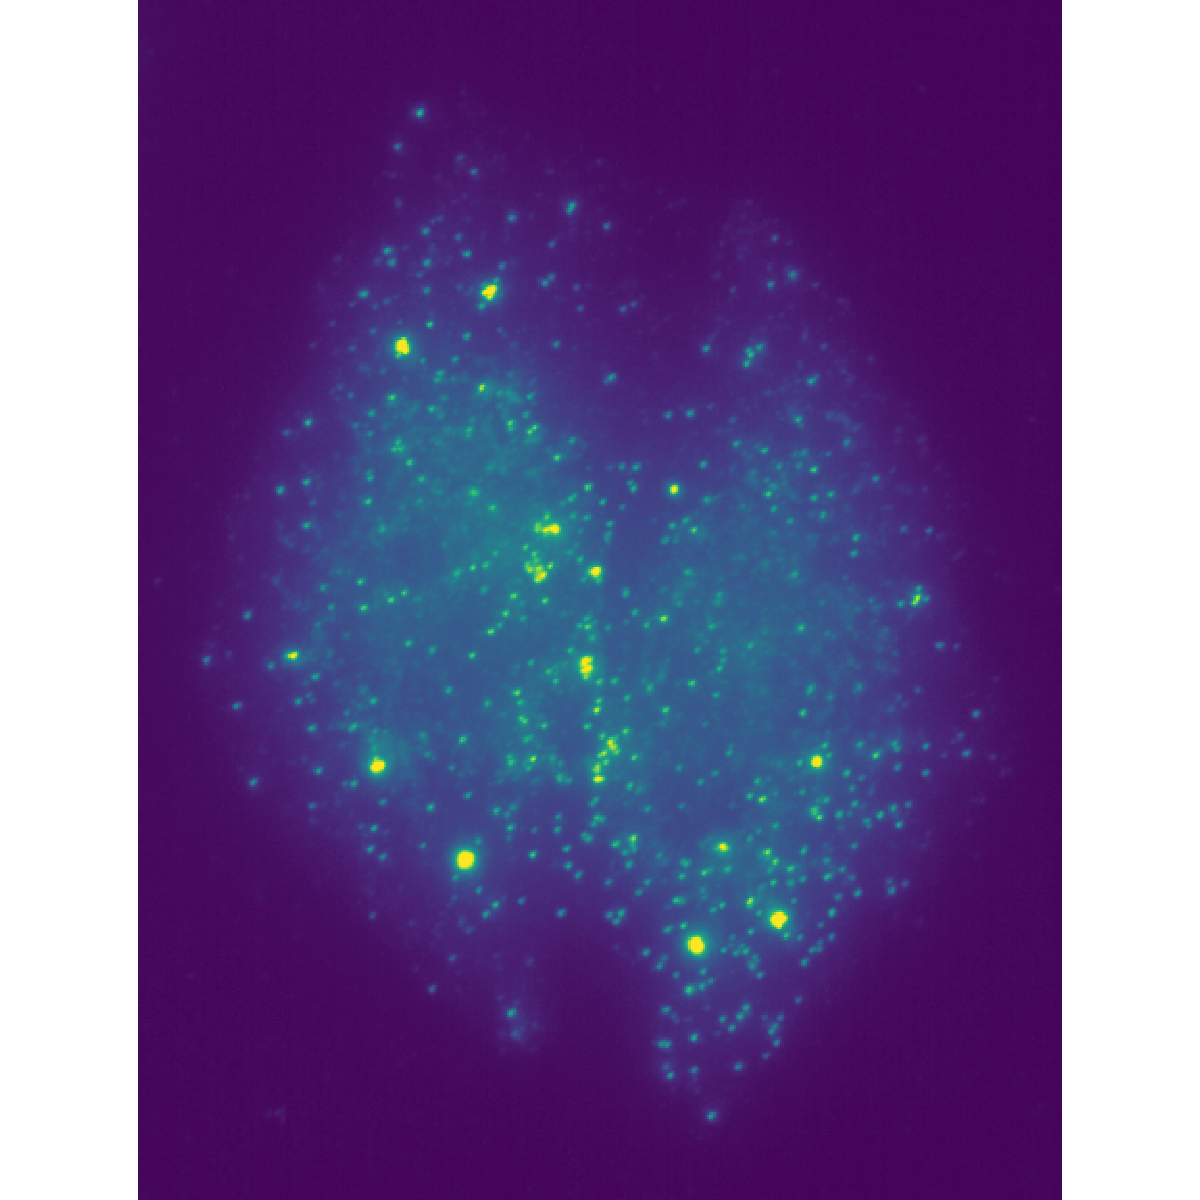
\includegraphics[width=\textwidth]{figures/introduction/multichannel_input}
    \caption[Example of DAPI and smiFISH images]{Example of DAPI (\textit{left}) and smiFISH (\textit{right}) images}
    \label{fig:multichannel_input}
\end{figure}

\subsection{Fluorescent proteins}
\label{subsec:intro_fluorescence}

\subsection{A zoo of FISH}
\label{subsec:intro_fish}

%%%%%%%%%%%%%%%%%%%%%%%%%%%%%%%%%%%%%%%%%%%%%%%%%%%%%%%%%%%%%%%%%%%%%%%%%%%%%%%%%%%%%%%%%%%%%%%%%%%%%%%%%%%%%%%%%%%%%%%%%%%%%%%%%%%%%%%%%%%%%%%%%%%%%%%%%%%%

% thesis adham: "the invention of single molecule FISH (Femino et al., 1998)"

%%%%%%%%%%%%%%%%%%%%%%%%%%%%%%%%%%%%%%%%%%%%%%%%%%%%%%%%%%%%%%%%%%%%%%%%%%%%%%%%%%%%%%%%%%%%%%%%%%%%%%%%%%%%%%%%%%%%%%%%%%%%%%%%%%%%%%%%%%%%%%%%%%%%%%%%%%%%

% paper racha (dual protein-rna localization screens)

% In order to simultaneously visualize mRNAs with their encoded proteins, we based our screen on a library of HeLa cell lines,
% each containing a bacterial artificial chromosome (BAC) stably integrated in their genome (Poser et al., 2008).
% Each BAC con- tains a GFP-tagged gene harboring all its regulatory sequences (promoter, enhancers, introns, and 50 and 30 UTRs; Figure 1A).
% The resulting mRNAs are, thus, identical to the endogenous mol- ecules in terms of sequence and isoform diversity, except for the added tag.
% Previous studies showed that such tagged genes are expressed at near endogenous levels and with the proper spatio- temporal pattern (Poser et al., 2008).
% Since the tagged mRNAs contain all the regulatory sequences, we hypothesized that they would localize like the endogenous ones,
% provided that the tag does not interfere with localization. Using BACs offers two advantages. First, a single smFISH probe set
% against the GFP sequence is sufficient to detect all the studied mRNAs. Sec- ond, using mild hybridization conditions,
% GFP fluorescence can be detected together with the smFISH signal (Fusco et al., 2003), and thus, both the mRNA and the encoded protein can be detected in the same cell.

%%%%%%%%%%%%%%%%%%%%%%%%%%%%%%%%%%%%%%%%%%%%%%%%%%%%%%%%%%%%%%%%%%%%%%%%%%%%%%%%%%%%%%%%%%%%%%%%%%%%%%%%%%%%%%%%%%%%%%%%%%%%%%%%%%%%%%%%%%%%%%%%%%%%%%%%%%%%

\begin{wrapfigure}{R}{0.60\textwidth}
	\begin{center}
	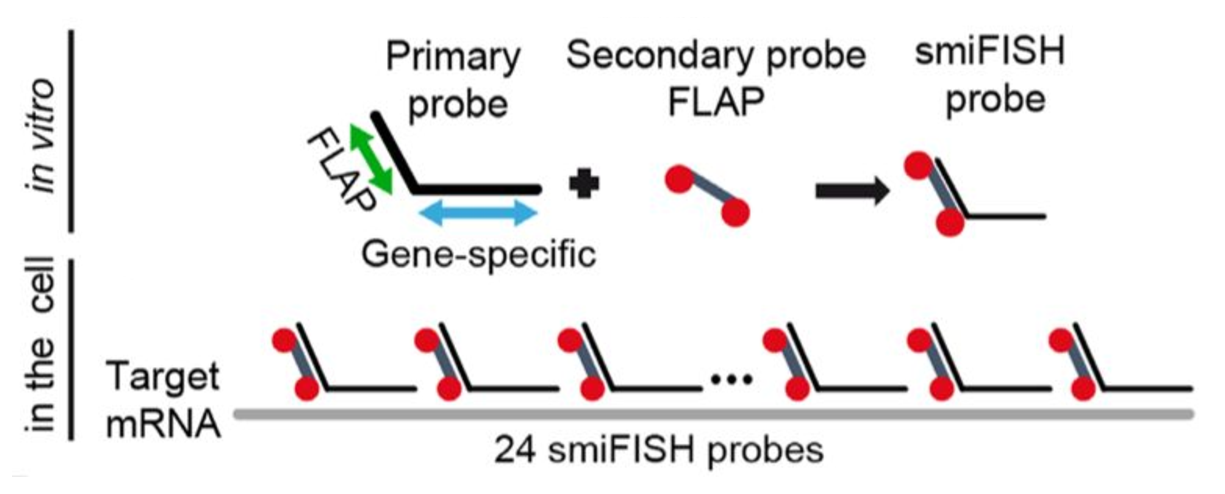
\includegraphics[width=\linewidth]{figures/introduction/smiFISH}
	\caption[Schema of smiFISH protocol]{Schema of smiFISH protocol from~\cite{tsanov_smifish_2016}}
	\label{fig:smiFISH}
	\end{center}
\end{wrapfigure}

%%%%%%%%%%%%%%%%%%%%%%%%%%%%%%%%%%%%%%%%%%%%%%%%%%%%%%%%%%%%%%%%%%%%%%%%%%%%%%%%%%%%%%%%%%%%%%%%%%%%%%%%%%%%%%%%%%%%%%%%%%%%%%%%%%%%%%%%%%%%%%%%%%%%%%%%%%%%
%%%%%%%%%%%%%%%%%%%%%%%%%%%%%%%%%%%%%%%%%%%%%%%%%%%%%%%%%%%%%%%%%%%%%%%%%%%%%%%%%%%%%%%%%%%%%%%%%%%%%%%%%%%%%%%%%%%%%%%%%%%%%%%%%%%%%%%%%%%%%%%%%%%%%%%%%%%%
%%%%%%%%%%%%%%%%%%%%%%%%%%%%%%%%%%%%%%%%%%%%%%%%%%%%%%%%%%%%%%%%%%%%%%%%%%%%%%%%%%%%%%%%%%%%%%%%%%%%%%%%%%%%%%%%%%%%%%%%%%%%%%%%%%%%%%%%%%%%%%%%%%%%%%%%%%%%

\section{Measuring images: from pixels to numbers}
\label{sec:computation_biology}

\begin{center}
	\textit{(To be completed)}
\end{center}

\subsection{Working with images}
\label{subsec:intro_images}

% specificity to bioimage
% from pixels to numbers

\begin{figure}[]
	\centering
	\minipage{0.2\textwidth}
		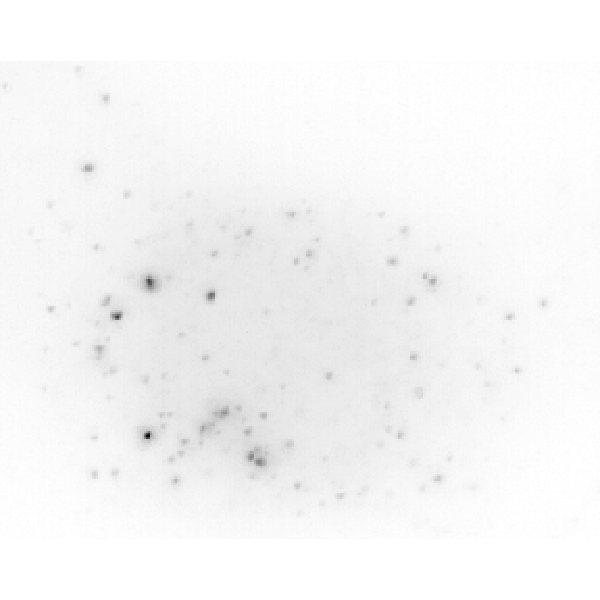
\includegraphics[width=0.95\linewidth]{figures/introduction/real_image_foci}
		\vfill
		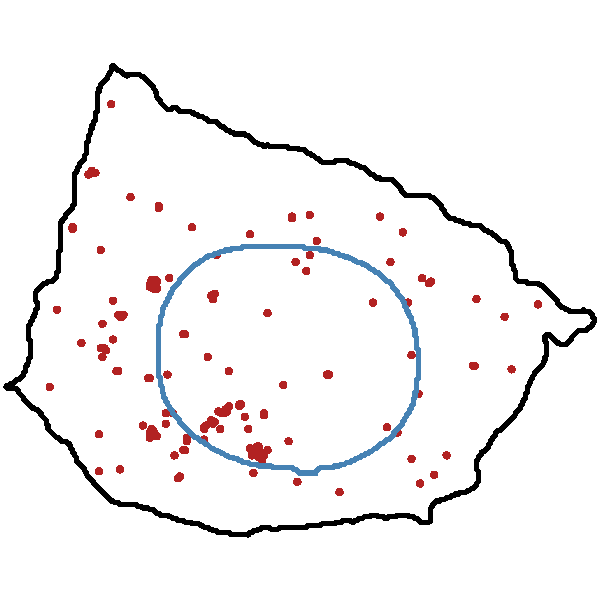
\includegraphics[width=0.95\linewidth]{figures/introduction/real_coord_foci}
		\subcaption{Foci}
	\endminipage\hfill
	\minipage{0.2\textwidth}
		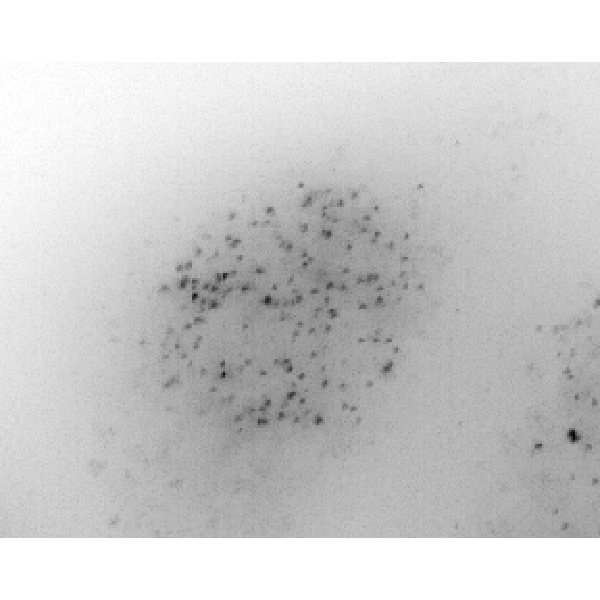
\includegraphics[width=0.95\linewidth]{figures/introduction/real_image_intranuclear}
		\vfill
		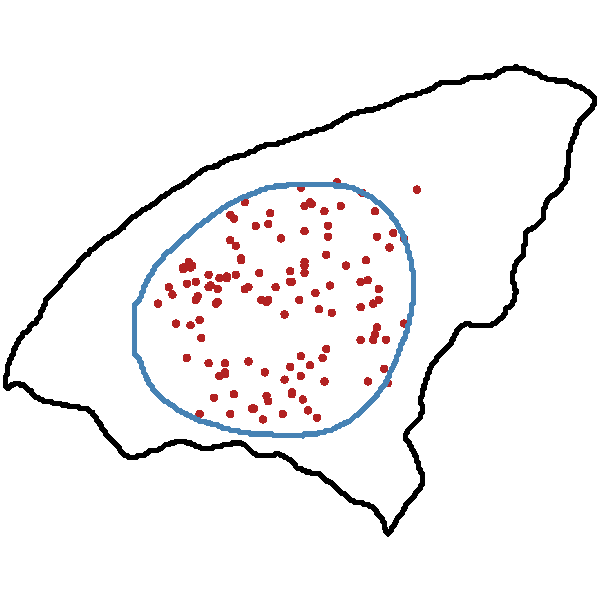
\includegraphics[width=0.95\linewidth]{figures/introduction/real_coord_intranuclear}
		\subcaption{Intranuclear}
	\endminipage\hfill
	\minipage{0.2\textwidth}
		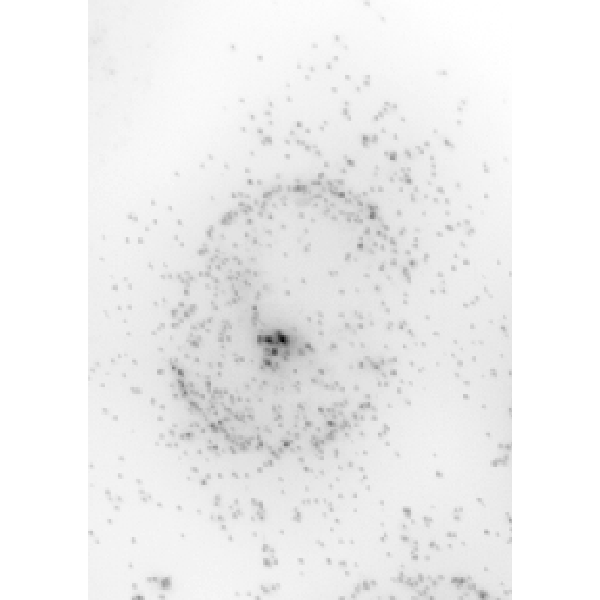
\includegraphics[width=0.95\linewidth]{figures/introduction/real_image_nuclear_edge}
		\vfill
		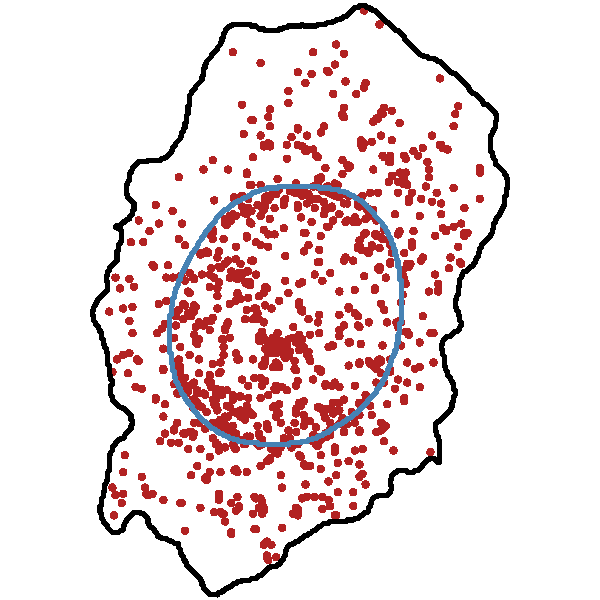
\includegraphics[width=0.95\linewidth]{figures/introduction/real_coord_nuclear_edge}
		\subcaption{Nuclear edge}
	\endminipage\hfill
	\minipage{0.2\textwidth}
		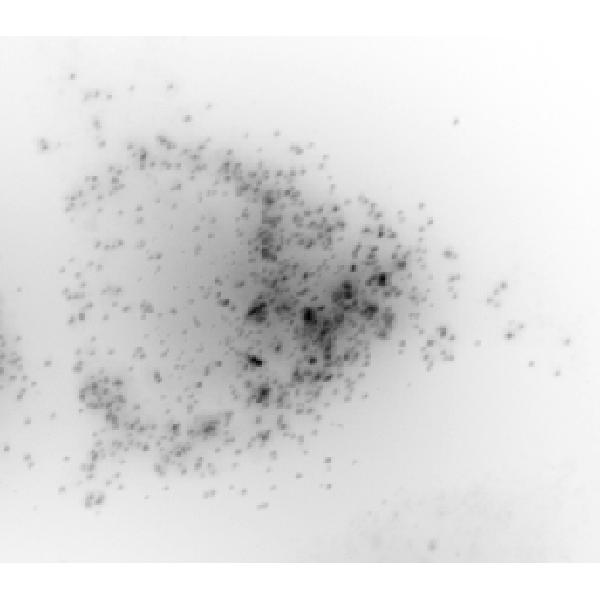
\includegraphics[width=0.95\linewidth]{figures/introduction/real_image_perinuclear}
		\vfill
		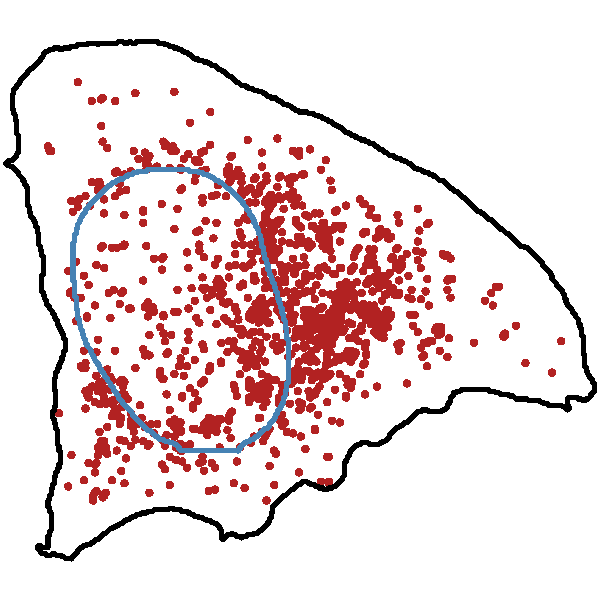
\includegraphics[width=0.95\linewidth]{figures/introduction/real_coord_perinuclear}
		\subcaption{Perinuclear}
	\endminipage\hfill
	\minipage{0.2\textwidth}
		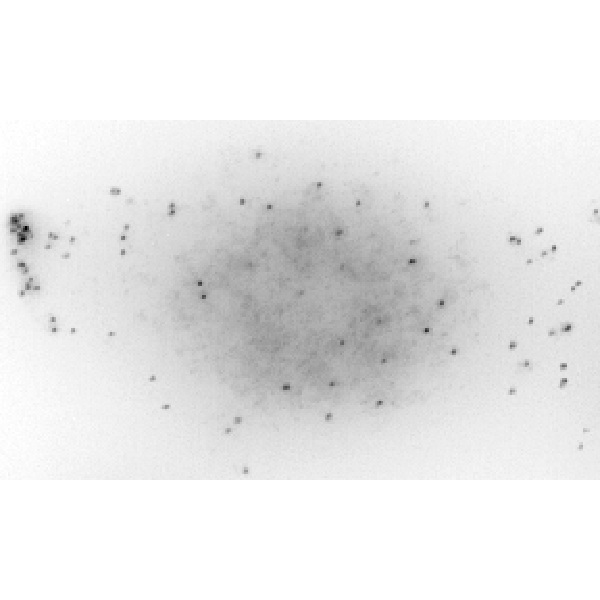
\includegraphics[width=0.95\linewidth]{figures/introduction/real_image_protrusion}
		\vfill
		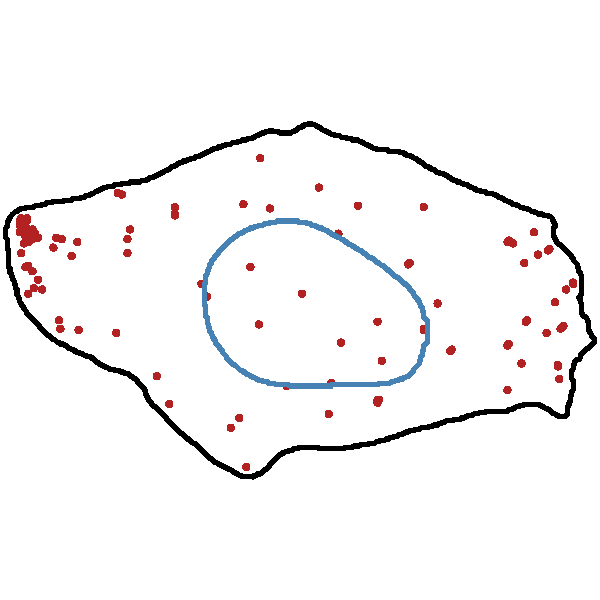
\includegraphics[width=0.95\linewidth]{figures/introduction/real_coord_protrusion}
		\subcaption{Protrusion}
	\endminipage
	\caption[RNA localization patterns: from pixels to numbers]{RNA localization patterns from~\cite{pointfish_2022}.
	(\textit{Top}) Typical smFISH images with different RNA localization patterns.
	(\textit{Bottom}) Coordinate representations with RNA spots (red), cell membrane (black) and nuclear membrane (blue).
	Detection and segmentation results are extracted and visualized with FISH-quant~\cite{Imbert_fq_2022}}
	\label{fig:intro_localization_patterns}
\end{figure}

\subsection{A machine learning boom}
\label{subsec:intro_ml_tools}

% learning principles + generic modules of deep learning + flexible architecture
% advantage/limitations over traditionnal methods -> need to train (heterogeneity of dataset // self or weaekly supervised methods, simulations)
% caveats + evaluation (varoquaux)

%~\cite{lecun_deep_2015}

%%%%%%%%%%%%%%%%%%%%%%%%%%%%%%%%%%%%%%%%%%%%%%%%%%%%%%%%%%%%%%%%%%%%%%%%%%%%%%%%%%%%%%%%%%%%%%%%%%%%%%%%%%%%%%%%%%%%%%%%%%%%%%%%%%%%%%%%%%%%%%%%%%%%%%%%%%%%
%%%%%%%%%%%%%%%%%%%%%%%%%%%%%%%%%%%%%%%%%%%%%%%%%%%%%%%%%%%%%%%%%%%%%%%%%%%%%%%%%%%%%%%%%%%%%%%%%%%%%%%%%%%%%%%%%%%%%%%%%%%%%%%%%%%%%%%%%%%%%%%%%%%%%%%%%%%%
%%%%%%%%%%%%%%%%%%%%%%%%%%%%%%%%%%%%%%%%%%%%%%%%%%%%%%%%%%%%%%%%%%%%%%%%%%%%%%%%%%%%%%%%%%%%%%%%%%%%%%%%%%%%%%%%%%%%%%%%%%%%%%%%%%%%%%%%%%%%%%%%%%%%%%%%%%%%

\section{Goals and contributions}
\label{sec:contributions}

\subsection{Goals}
\label{subsec:intro_goals}

At the beginning of my PhD, three main goals were defined with my supervisors.
The first one was the development and the implementation of a complete pipeline to process \ac{smFISH} images and return valuable insights about \ac{RNA} localization.
In particular, it was expected to integrate and adapt the latest successful developments in computer vision.
The second goal was the identification of bottlenecks that would prevent scaling the analysis to thousands images, in high content screening assays.
Such bottlenecks should be minimized or solved during the thesis to be able to scale any computational analysis based on \ac{smFISH} experiments.
Lastly, this complete framework would be applied to real experimental datasets in ongoing biological studies.

\subsection{Contributions}
\label{subsec:intro_contributions}

Beyond this own manuscript, my contributions are essentially lines of code.
With a effort of transparency, reproducibility and documentation, I try to develop computational tools as useful as possible for any biologist interested in \ac{FISH} experiments.
My PhD results in three major contributions.

\begin{itemize}
	\setlength\itemsep{0.1em}
	\item My first and main contribution is FISH-quant V2.
	This online framework gathers Python packages and a \ac{GUI} to process \ac{FISH} images, build robust analysis pipelines and even perform simulations.
	\item My second important contribution is an alternative method to compute relevant features in order to discriminate \ac{RNA} localization patterns.
	This method implies the development of PointFISH, a dedicated deep learning model for point cloud.
	\item My third contribution is my participation to biological studies with meaningful results.
	These studies leveraged high content screening assays and \ac{smFISH} techniques to perform a systemic analysis of \ac{RNA} localization and investigate local translation phenomenons.
\end{itemize}

\noindent
Some other contributions are also mentioned throughout this manuscript.
It includes a dataset I annotated for nucleus and cell segmentation with thousands of instances and my supervision of an intern.
The work performed during this internship was the seed for the first publication of another PhD student in the team, about in silico labeling and segmentation.
Lastly, a list of my publications are available at the very end of the manuscript.

\subsection{Manuscript summary}
\label{subsec:intro_manuscript}

The manuscript is composed of two parts.
The first four chapters are a presentation of the analysis pipeline with a focus on every critical stage.
It includes systematic reviews of the existing methods and details about solutions I implemented.
In addition, code snippets, ready to be imported and run, are interspersed with descriptions of the related algorithms.
The second part details several applications of my tools, where quantification of \ac{RNA} localization patterns supports biological insights.

In \textbf{Chapter~\ref{ch:chapter1}}, I present the general computational framework I developed and published: FISH-quant v2.
It includes methods for every stages of a \ac{FISH}-based analysis, with an effort to make them scalable and modular.
I also describe the improvements from the original FISH-quant version, and how it addresses the requirements of a modern software tool.

In \textbf{Chapter~\ref{ch:chapter2}}, I focus on the \ac{RNA} detection stage.
With \ac{smFISH} experiments, the \ac{RNA} molecules are spotted and reduced to discrete data points in space.
I describe detection algorithms and their extensions available in FISH-quant.
In the end, the set of all \ac{RNA} molecules is reduced to a point cloud with spatial coordinates.

In \textbf{Chapter~\ref{ch:chapter3}}, I review and describe algorithms for nucleus and cell segmentation.
Most of them are deep learning models, trained on vast datasets of annotated images.
Beside my own implemented methods, I also present refinement techniques to improve and format segmentation masks.
Two other projects for which I contributed (including one published) are also discussed at the end of the chapter.
They aim at improving the efficiency and consistency of segmentation on specific aspects.

In \textbf{Chapter~\ref{ch:chapter4}}, I compare two different approaches to quantify \ac{RNA} localization patterns.
Once the \ac{RNA} molecules are detected and cell morphology is segmented, the pixel domain gives way to Euclidean space and cells can be represented with a coordinate representation.
Then, spatial features are computed in order to discriminate relevant localization pattern.
I present two different methods of feature engineering.
The first method consists in manually designing features to characterize specific localization patterns.
I then list and describe every hand-crafted feature implemented in FISH-quant.
The second (published) method consists in learning features.
They are extracted from a deep learning model fed with the \ac{RNA} point cloud as input and trained on a simulated pretext task.

In \textbf{Chapter~\ref{ch:chapter5}}, I present several applications of my quantitative pipeline.
These applications come from three publications where we study different \ac{RNA} localization patterns and cases of local translation.
My analyses support and validates biological insights claimed in these studies about \ac{RNA} localization.
I design a classification pipeline to recognize generic localization patterns.
I evaluate the impact of translation inhibitor on \ac{RNA} localization and help identifying a singular translation-dependent pattern.
I quantify a cell cycle dependent pattern, which is related to centrosomes.
Finally, I also contribute to a a study focused on the protrusion pattern.

%%%%%%%%%%%%%%%%%%%%%%%%%%%%%%%%%%%%%%%%%%%%%%%%%%%%%%%%%%%%%%%%%%%%%%%%%%%%%%%%%%%%%%%%%%%%%%%%%%%%%%%%%%%%%%%%%%%%%%%%%%%%%%%%%%%%%%%%%%%%%%%%%%%%%%%%%%%%
%%%%%%%%%%%%%%%%%%%%%%%%%%%%%%%%%%%%%%%%%%%%%%%%%%%%%%%%%%%%%%%%%%%%%%%%%%%%%%%%%%%%%%%%%%%%%%%%%%%%%%%%%%%%%%%%%%%%%%%%%%%%%%%%%%%%%%%%%%%%%%%%%%%%%%%%%%%%
%%%%%%%%%%%%%%%%%%%%%%%%%%%%%%%%%%%%%%%%%%%%%%%%%%%%%%%%%%%%%%%%%%%%%%%%%%%%%%%%%%%%%%%%%%%%%%%%%%%%%%%%%%%%%%%%%%%%%%%%%%%%%%%%%%%%%%%%%%%%%%%%%%%%%%%%%%%%

% plots

% (RNA maturation)
% RNA transport mechanism

% smFISH + microscope
% multichannel images (dapi + smfish)
% multiplexed FISH

% (deep learning architecture)

% add presentation of the localization patterns (from pixel to coord + patterns)
% mention Weeks et al. (1985) as firstpublication about RNA localization
% adham thesis: "Messenger localization was first discovered in Xenopus oocytes (Weeks et al., 1985)."


%%%%%%%%%%%%%%%%%%%%%%%%%%%%%%%%%%%%%%%%%%%%%%%%%%%%%%%%%%%%%%%%%%%%%%%%%%%%%%%%%%%%%%%%%%%%%%%%%%%%%%%%%%%%%%%%%%%%%%%%%%%%%%%%%%%%%%%%%%%%%%%%%%%%%%%%%%%%

% paper racha (introduction)

%how
%- rna metabolism
%- protein metabolism (mature protein or nascent protein)

%why
%- storage of untranslated rna
%- local translation
%- rapid cell division cycle (linked to local translation of cyclin B mRNAs)
%- cell polarization
%- cell motility (actin at the leading edge)
%- axonal growth and synaptic plasticity of neurons
%- assembly of protein complexes
%- avoid proteins in wrong place

%how
%- targeting signal of nascent protein
%- targeting from rna zip-code sequence (with RNA-binding proteins)
%- direct transport on the cytoskeleton by molecular motors
%- anchoring mechanism
%- diffusion, trapping, degradation and local rna stabilization

%claim
%- lack a global view of local translation in the entire cellular space or at the genomic level
%- need a systematic manner

%examples
%- pioneering study in Drosophila
%- human cell lines

%limitations
%- information on RNA localization but did not directly investigate local translation as the encoded proteins were not detected

%%%%%%%%%%%%%%%%%%%%%%%%%%%%%%%%%%%%%%%%%%%%%%%%%%%%%%%%%%%%%%%%%%%%%%%%%%%%%%%%%%%%%%%%%%%%%%%%%%%%%%%%%%%%%%%%%%%%%%%%%%%%%%%%%%%%%%%%%%%%%%%%%%%%%%%%%%%%

% paper racha (introduction)

% Most mRNAs are distributed randomly throughout the cytoplasm, but some localize to specific
% subcellular areas (Blower, 2013; Bovaird et al., 2018; Eliscovich and Singer, 2017; Jung et al., 2014 for reviews).

% This phenomenon is linked to either RNA metabolism, when untranslated mRNAs are stored in P- bodies or other cellular structures (Hubstenberger et al., 2017),
% or to protein metabolism, when a protein is synthesized locally.

% Local translation has been observed from bacteria and yeast to humans (Blower, 2013; Jung et al., 2014; Eliscovich and Singer, 2017; Bovaird et al., 2018).

% It is commonly involved in the delivery of mature proteins to specific cellular compartments, while allowing local regulation, and this is involved in many processes.
% For instance, it contributes to patterning and cell fate determination during metazoan development, mainly through asymmetric cell division
% (Melton, 1987; Driever and Nu€sslein- Volhard, 1988).
% In Xenopus embryos, local translation of cyclin B mRNAs at the mitotic spindle is also believed to be important for the rapid cell
% division cycles occurring during early embryo- genesis (Groisman et al., 2000).
% In mammals, mRNA localization is involved in cell polarization and motility, mainly through the localization of actin and related mRNAs at the leading edge (Lawrence and Singer, 1986), and it is also involved in axonal
% growth and synaptic plasticity of neurons (Van Driesche and Martin, 2018).

% Importantly, local translation can also be linked to the
% metabolism of the nascent peptide rather than to directly localize the mature protein. For instance, translation of secreted proteins
% at the endoplasmic reticulum (ER) allows nascent pro- teins to translocate through the membrane to reach the ER lumen (Aviram and Schuldiner, 2017).
% Translation of mRNAs at specific sites may also be important for the assembly of protein complexes (Pichon et al., 2016) or
% to avoid the deleterious effects of releasing free proteins at inappropriate places (Mu€ller et al., 2013).

% RNA localization can be accomplished through several mech- anisms. In the case of secreted proteins, the nascent peptide serves as a
% targeting signal, via the signal recognition particle (SRP) and its receptor on the ER (Aviram and Schuldiner, 2017).

% In most other cases, targeting is an RNA-driven process (Blower, 2013; Jung et al., 2014; Eliscovich and Singer, 2017; Bovaird et al., 2018 for reviews).
% Localized mRNAs often contain a zip-code sequence, frequently located within their 30-UTR, which is necessary and sufficient to transport them to their destination.
% The zip code is recognized by one or several RNA-binding proteins (RBPs), and it drives the formation of a transport complex sometimes called locasome.
% This complex can be transported by centrosomes, endosomal vesicles, or other cellular structures (Blower, 2013; Jung et al., 2014; Eliscovich and Singer, 2017; Bovaird et al., 2018).

% However, direct transport on the cytoskeleton by molecular motors is a frequent mechanism (Blower, 2013; Bovaird et al., 2018; Eliscovich and Singer, 2017; Jung et al., 2014).

% Once at destination, an anchoring mechanism may limit diffusion away from the target site.

% Alternatives to these transport mechanisms include diffusion and trap- ping at specific locations and degradation coupled to local RNA stabilization.

% Localized mRNAs are often subjected to a spatial control of translation (Besse and Ephrussi, 2008).
% In the case of Ash1 mRNA in yeast and b-actin mRNA in neurons, translation is repressed during transport and
% is activated at their final location by phosphorylation-dependent mechanisms (Hu€ttelmaier et al., 2005; Paquin et al., 2007).
% This spatial regulation of translation provides an additional layer of control ensuring that mRNAs are translated only at the desired location.

% The first locally translated mRNAs were found by chance or using a candidate approach.
% Purification of cellular structures and localized RBPs have significantly increased the number of known localized mRNAs
% (Blower, 2013; Jung et al., 2014; Eliscovich and Singer, 2017; Bovaird et al., 2018).

% However, only specific compartments or RBPs were examined, and we currently lack a global view of local translation in the entire cellular space or at the genomic level.
% Few reports described attempts to characterize mRNA localization in a systematic manner.

% A pioneering study in Drosophila used whole-mount fluorescent in situ hybrid- ization (FISH) to analyze the localization of more than 2,000 mRNAs (Lecuyer et al., 2007).
% As many as 71\% of them had a non-random distribution, and a range of new localization patterns were observed.
% More recent reports confirmed that RNA localization is widespread during Drosophila development (Jam- bor et al., 2015; Wilk et al., 2016).

% However, it is not known whether this is also true in other organisms, particularly in humans. Few recent studies addressed this question in cell lines
% using the more sensitive single-molecule FISH technique (smFISH). Several thousands of mRNAs were analyzed, which
% showed a correlation of intracellular mRNA distribution with gene annotation (Battich et al., 2013; Chen et al., 2015; Eng et al., 2019; Xia et al., 2019).
% Specifically, these studies identified three groups of localized mRNAs, in the perinuclear area, the mitochondria, and the cell periphery,
% the latter being possibly linked to actin metabolism (Chen et al., 2015).

% These studies provided information on RNA localization but did not directly investigate local translation as the encoded proteins were not detected.
% Thus, we still lack a good understanding of the various functions played by local translation at the cellular level.

% In this study, we developed a smFISH screen to specifically address this issue. Using a set of 523 GFP-tagged cell lines spanning
% a variety of cellular functions and an approach that allows simultaneous visualization of mRNA and proteins,
% we found that local translation occurs at various unanticipated locations. In particular, we discovered specialized
% translation factories, where specific mRNAs are translated. These factories are remarkable in that they provide
% a unique mean to regulate the metabolism of nascent proteins and also create a fine granular compartmentalization of translation.

%%%%%%%%%%%%%%%%%%%%%%%%%%%%%%%%%%%%%%%%%%%%%%%%%%%%%%%%%%%%%%%%%%%%%%%%%%%%%%%%%%%%%%%%%%%%%%%%%%%%%%%%%%%%%%%%%%%%%%%%%%%%%%%%%%%%%%%%%%%%%%%%%%%%%%%%%%%%
